

\begin{figure}[tb]
  \begin{center}
    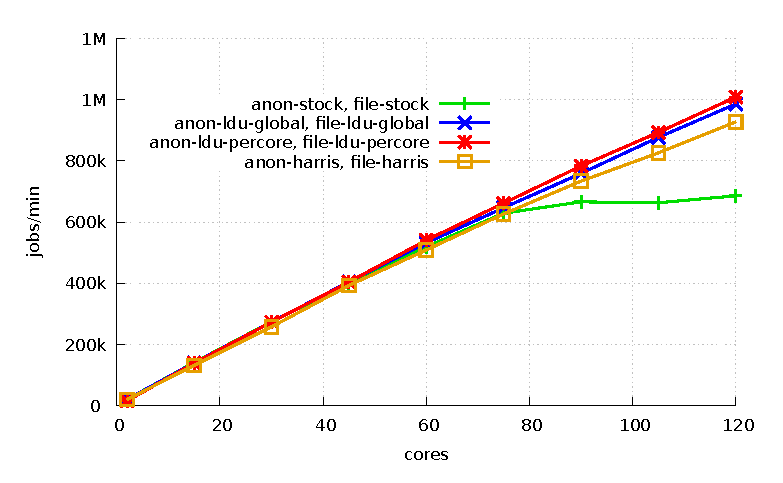
\includegraphics[scale=0.8]{graph/aim7.eps}
  \end{center}
  \caption{Scalability of AIM7-multiuser.}
  \label{fig:aim7}
\end{figure}

\section{Evaluation}
\label{sec:evaluation}


\begin{figure*}[tb]
    \centering
    \begin{subfigure}[b]{1\textwidth}
  \begin{center}
        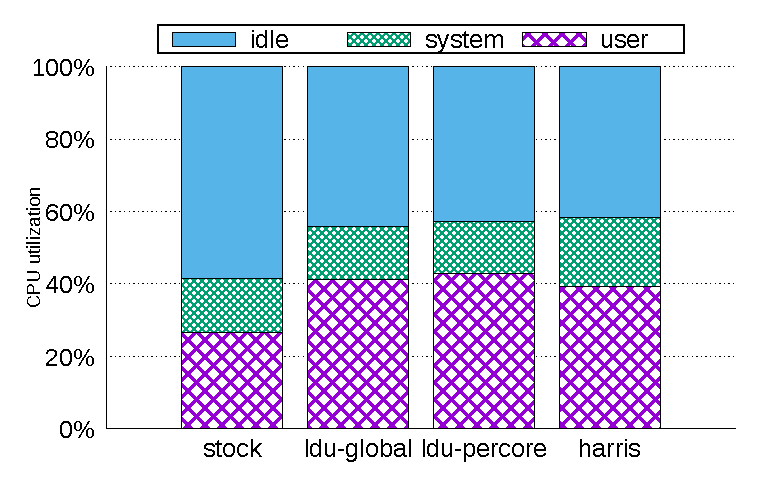
\includegraphics[scale=0.8]{graph/aim7_cpuutils.eps}
        \caption{AIM7 - 120core}
  \end{center}
    \end{subfigure}%
    \centering
    \caption{AIM7 CPU utilization on 120 core.}
    \label{fig:utilization_aim7}
    
\end{figure*}


\begin{figure*}[tb]
    \centering
    \begin{subfigure}[b]{1\textwidth}
  \begin{center}
        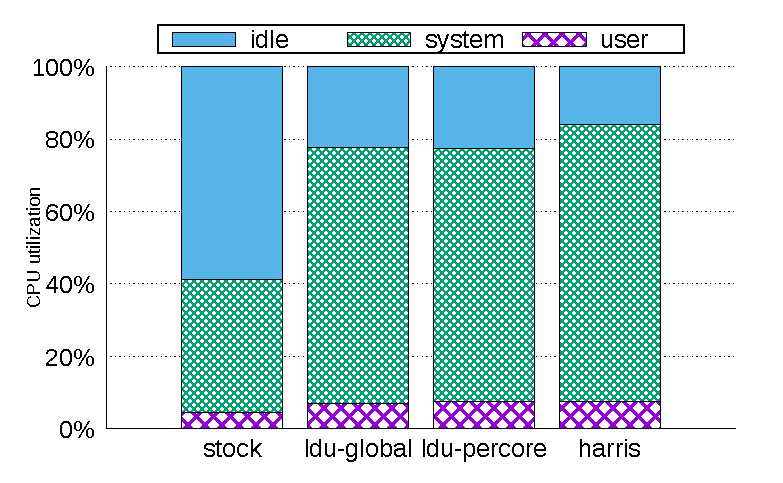
\includegraphics[scale=0.8]{graph/exim_cpuutils.eps}
        \caption{Exim - 120core}
  \end{center}
    \end{subfigure}
    \centering
    \caption{EXIM CPU utilization on 120 core. }
    \label{fig:utilization_exim}
    
\end{figure*}



\begin{figure*}[tb]
    \centering
    \begin{subfigure}[b]{1\textwidth}
  \begin{center}
        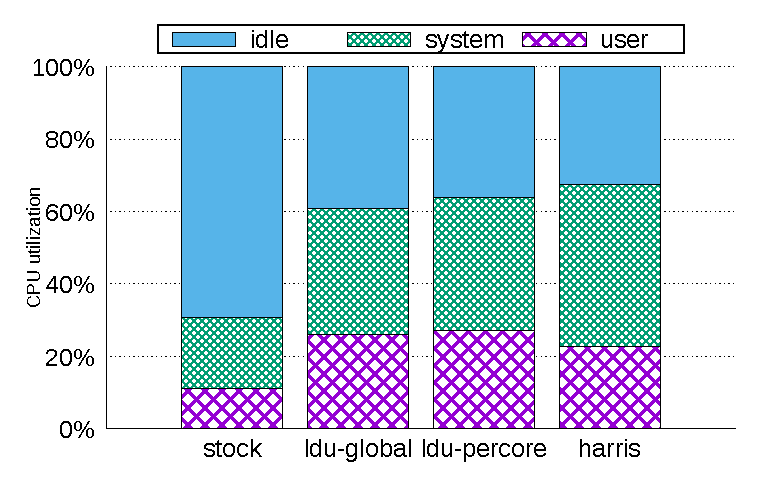
\includegraphics[scale=0.8]{graph/lmbench_cpuutils.eps}
        \caption{Lmbench - 120core}
  \end{center}
    \end{subfigure}
        \centering
    \caption{Lmbench CPU utilization on 120 core.}
    \label{fig:utilization_lmbench}
    
\end{figure*}



\subsection{Experimental setup}

%$$$$$$$$$$$$$$$$$$$$$$$$$$$$$$$$$$$$$$$$$$$$$$$$$$$$$$$$$$$$$$$$$$$$$$$$$$$$$$$$
%Paragraph 1: 무엇을 평가 했는지에 대한 설명 
%$$$$$$$$$$$$$$$$$$$$$$$$$$$$$$$$$$$$$$$$$$$$$$$$$$$$$$$$$$$$$$$$$$$$$$$$$$$$$$$$

For the purpose of performance evaluation of the proposed 
\LDU technique, we performed experiments using a Linux kernel
where \LDU technique is implemented compared to a lock-free list
version of Linux proposed by Harris~\cite{Harris2001Lockfree}.
The reason why we used Harris algorithm for our comparison 
purposes is that the algorithm is considered as the representative
concurrent non-blocking algorithm.
The basic algorithms of Harris linked list are from sysnchrobench~\cite{Gramoli2015Synchrobench}
and ASCYLIB~\cite{David2015ASYNCHRONIZED}, and we slightly converted the
Harris linked list to be adopted in Linux kernels.

%$$$$$$$$$$$$$$$$$$$$$$$$$$$$$$$$$$$$$$$$$$$$$$$$$$$$$$$$$$$$$$$$$$$$$$$$$$$$$$$$
%Paragraph 3: 운영체제 및 커널 버전 설명
%$$$$$$$$$$$$$$$$$$$$$$$$$$$$$$$$$$$$$$$$$$$$$$$$$$$$$$$$$$$$$$$$$$$$$$$$$$$$$$$$
The hardware specification we used for our experiments
are a 120 core machine with 8-socket, Intel
E7-8870 chips(15 cores per socket) equipped with 792 GB DDR3 DRAM.

%$$$$$$$$$$$$$$$$$$$$$$$$$$$$$$$$$$$$$$$$$$$$$$$$$$$$$$$$$$$$$$$$$$$$$$$$$$$$$$$$
%Paragraph 2-1: Harris Lock free list 구현 내용에 대한 설명 
%$$$$$$$$$$$$$$$$$$$$$$$$$$$$$$$$$$$$$$$$$$$$$$$$$$$$$$$$$$$$$$$$$$$$$$$$$$$$$$$$
%To compare our the \LDU implementation to a concurrent non-blocking
%algorithm, we additionally implemented the
%Harris linked list~\cite{Harris2001Lockfree} to Linux kernel.
%The Harris linked list refers from sysnchrobench~\cite{Gramoli2015Synchrobench}
%and ASCYLIB~\cite{David2015ASYNCHRONIZED}, and we slightly converted the
%Harris linked list to the Linux kernel style.
%Then, we replaced the two interval tree to the Harris linked list.
%In addition, since the Harris linked list in the synchrobench and the ASCYLIB leaks memory,
%we implemented a garbage collector for Linux kernel using the Linux work
%queues and non-blocking linked list.

%$$$$$$$$$$$$$$$$$$$$$$$$$$$$$$$$$$$$$$$$$$$$$$$$$$$$$$$$$$$$$$$$$$$$$$$$$$$$$$$$
%Paragraph 1: 벤치 마크 대한 설명
%$$$$$$$$$$$$$$$$$$$$$$$$$$$$$$$$$$$$$$$$$$$$$$$$$$$$$$$$$$$$$$$$$$$$$$$$$$$$$$$$
We selected benchmark programs with fork-intensive applications since the fork-intensive update-heavy data structure accesses could maximally benefit from the proposed technique.
The benchmark programs are AIM7, a Linux
scalability benchmark, Exim, an email server in MOSBENCH, and Lmbench, a micro benchmark.
The workloads exhibit the high lock contentions because of the two reverse mappings.
Moreover, the AIM7 benchmark is widely used in the Linux community not only for
testing Linux kernel but also for improving the scalability. 
The Exim is a real world application, but it has scalability bottlenecks caused
by the Linux fork.
Finally, in order to only focus on the fork performance and scalability, we
selected the Lmbench.

%$$$$$$$$$$$$$$$$$$$$$$$$$$$$$$$$$$$$$$$$$$$$$$$$$$$$$$$$$$$$$$$$$$$$$$$$$$$$$$$$
%Paragraph 2: 비교 대상에 대한 설명
%$$$$$$$$$$$$$$$$$$$$$$$$$$$$$$$$$$$$$$$$$$$$$$$$$$$$$$$$$$$$$$$$$$$$$$$$$$$$$$$$
We used four different experiment settings. 
First, we used the stock Linux as the baseline reference. 
Second, we used the \LDU version of Linux kernel that used global queue.
Next, we used the per-core queue version of the \LDU.
Finally, we used Harris lock-free list version of Linux kernel as we
mentioned earlier.
Unfortunately, direct comparison experiments between the \LDU and the OpLog was not possible for a few implementation-related issues
(e.g., we could not obtain the detailed implementation of the OpLog).

\subsection{AIM7}

%$$$$$$$$$$$$$$$$$$$$$$$$$$$$$$$$$$$$$$$$$$$$$$$$$$$$$$$$$$$$$$$$$$$$$$$$$$$$$$$$
%Paragraph 1: AIM7 실험 결과
%$$$$$$$$$$$$$$$$$$$$$$$$$$$$$$$$$$$$$$$$$$$$$$$$$$$$$$$$$$$$$$$$$$$$$$$$$$$$$$$$


%$$$$$$$$$$$$$$$$$$$$$$$$$$$$$$$$$$$$$$$$$$$$$$$$$$$$$$$$$$$$$$$$$$$$$$$$$$$$$$$$
%Paragraph 1: 워크로드에 대한 설명
%$$$$$$$$$$$$$$$$$$$$$$$$$$$$$$$$$$$$$$$$$$$$$$$$$$$$$$$$$$$$$$$$$$$$$$$$$$$$$$$$
We used AIM7-multiuser, which is one of fork-intensive workload in AIM7.
The multiuser workload simultaneously creates many processes with various
operations(see section~\ref{sec:bg}), and we used the temp filesystem to minimize the file
system bottleneck.
We increased a number of users in proportion to number of cores.
 
%$$$$$$$$$$$$$$$$$$$$$$$$$$$$$$$$$$$$$$$$$$$$$$$$$$$$$$$$$$$$$$$$$$$$$$$$$$$$$$$$
%Paragraph 2: 실험 결과에 대한 설명
%$$$$$$$$$$$$$$$$$$$$$$$$$$$$$$$$$$$$$$$$$$$$$$$$$$$$$$$$$$$$$$$$$$$$$$$$$$$$$$$$
The results for AIM7-multiuser are shown in Figure~\ref{fig:aim7}.
Up to 75 core, the stock Linux scales linearly and then serialized updates
become bottlenecks.
However, up to 120 core, the Harris and our \LDU scale well because
these workloads can concurrently execute update operations without the
reader-writer semaphores(\code{anon\_vma->rwsem}, \code{mapping->i\_mmap\_rwsem}).
The per-core queue version of the \LDU shows the best performance and
scalability outperforming stock Linux by 1.5x and Harris by
1.1x.
In addition, although the global queue version of the \LDU has the global CAS operation, it
also has high performance and scalability because the global CAS operations are
mitigated by two \LDU techniques;it had 2\% performance degradation compared with
per-core queue version of the \LDU.
Furthermore, the stock Linux shows the highest idle time(58\%)(see
figure~\ref{fig:utilization_aim7}) since it waits to acquire semaphore(i.e., \code{anon\_vma->rwsem}, \code{mapping->i\_mmap\_rwsem}).
Surprisingly, although two \LDU have higher idle time than the Harris version, the throughput shows higher than the Harris because of our efficient algorithm.
\begin{figure}[tb]
  \begin{center}
    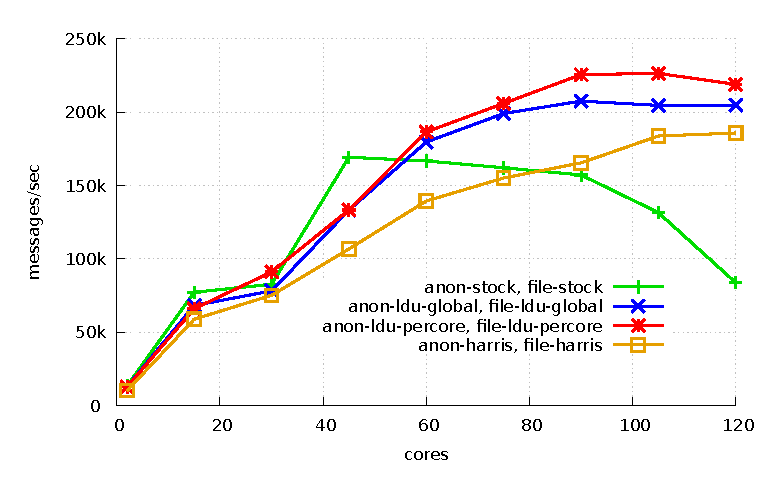
\includegraphics[scale=0.8]{graph/exim.eps}
  \end{center}
  \caption{Scalability of Exim.}
  \label{fig:exim}
\end{figure}

\subsection{Exim}
%$$$$$$$$$$$$$$$$$$$$$$$$$$$$$$$$$$$$$$$$$$$$$$$$$$$$$$$$$$$$$$$$$$$$$$$$$$$$$$$$
%Paragraph 1:  EXIM 실험 결과
%$$$$$$$$$$$$$$$$$$$$$$$$$$$$$$$$$$$$$$$$$$$$$$$$$$$$$$$$$$$$$$$$$$$$$$$$$$$$$$$$

\begin{figure}[tb]
  \begin{center}
    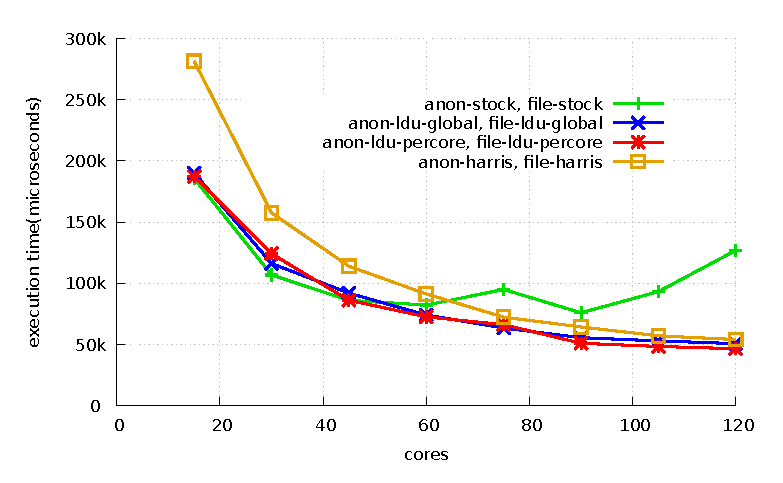
\includegraphics[scale=0.8]{graph/lmbench.eps}
  \end{center}
  \caption{Execution time of the process management workload in the Lmbench.}
  \label{fig:MicroBench}
\end{figure}

%$$$$$$$$$$$$$$$$$$$$$$$$$$$$$$$$$$$$$$$$$$$$$$$$$$$$$$$$$$$$$$$$$$$$$$$$$$$$$$$$
%Paragraph 1: 워크로드에 대한 설명
%$$$$$$$$$$$$$$$$$$$$$$$$$$$$$$$$$$$$$$$$$$$$$$$$$$$$$$$$$$$$$$$$$$$$$$$$$$$$$$$$
To measure the performance of the Exim, we used the MOSBENCH, a many-core
scalability benchmark.
The Exim email server is designed to scale because the Exim delivers messages to
mail boxes in parallel using the Linux process;the Exim is a fork-intensive
workload.
Clients ran on the same machine and each client sent to a different user to
prevent contention on user mail file.
The Exim was bottlenecked by the filesystem~\cite{SilasBoydWickizer2010LinuxScales48} since the message body appends to
the per-user mail file, so we used the separated tmpfs to reduce filesystem
bottlenecks.

%$$$$$$$$$$$$$$$$$$$$$$$$$$$$$$$$$$$$$$$$$$$$$$$$$$$$$$$$$$$$$$$$$$$$$$$$$$$$$$$$
%Paragraph 2:실험 결과에 대한 설명
%$$$$$$$$$$$$$$$$$$$$$$$$$$$$$$$$$$$$$$$$$$$$$$$$$$$$$$$$$$$$$$$$$$$$$$$$$$$$$$$$
Results shown in figure~\ref{fig:exim} indicate that the Exim scales well up to
60 core, but the stock Linux performance decreases near 60 core.
Both the Harris and the \LDU increase up to 105 core because they can execute
concurrent updates without the semaphores.
The per-core queue version of the \LDU performs better due to the fact that it can reduce
cache coherence-related overheads outperforming stock Linux by 2.6x and Harris
by 1.2x.
Even though we applied the scalable solutions, the Exim shows the limitation
near 105 core since the Exim process has a relatively large size of virtual
address mapping that leads to the clearing virtual address mappings overheads
and many soft page fault during the process destruction which executes more
slowly with more remote socket memory access.
The Harris has 15\% idle time, whereas per-core queue version of the \LDU
has 22\% idle time because the \LDU has the efficient algorithm(see
figure~\ref{fig:utilization_exim}).

\begin{figure*}[t!]
    \centering
    \begin{subfigure}[b]{1\textwidth}
  \begin{center}
        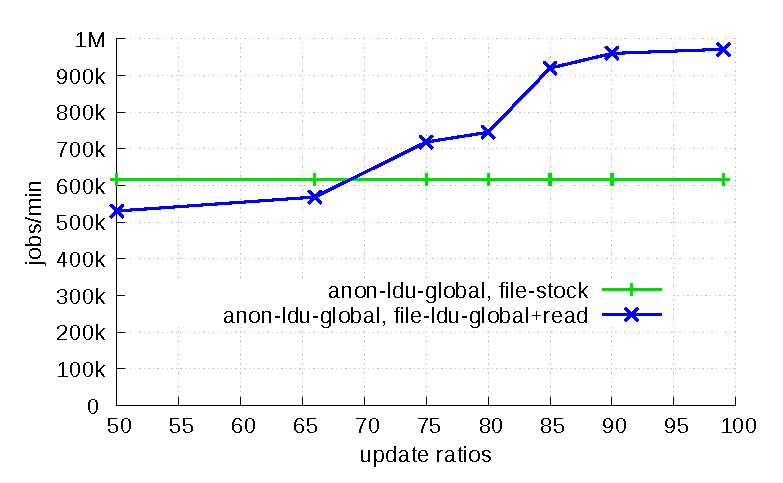
\includegraphics[height=2.5in]{graph/ratio_aim7.eps}
        \caption{AIM7 - 120core}
  \end{center}
    \end{subfigure}%
    \caption{Performance depending on update ratios and scalability.}
    \label{fig:UpdateRate_aim7}
\end{figure*}

\begin{figure*}[t!]
    \centering
    \begin{subfigure}[b]{1\textwidth}
        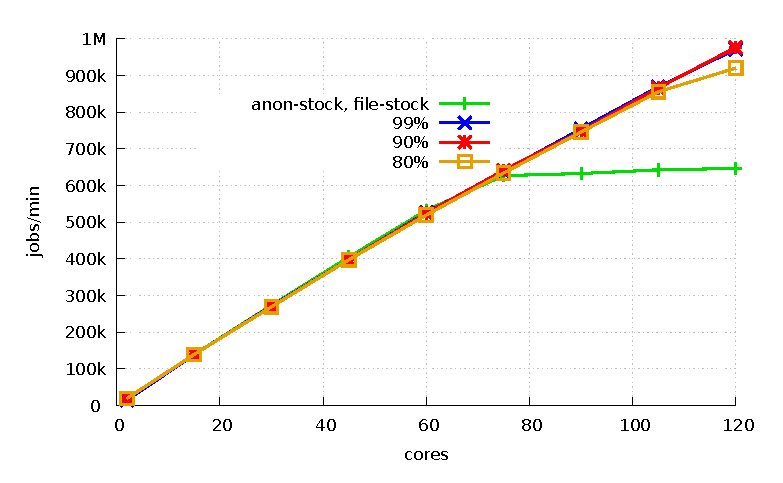
\includegraphics[height=2.5in]{graph/ratio_aim7_core.eps}
        \caption{AIM7 - scalability}
    \end{subfigure}%
    \caption{Performance depending on update ratios and scalability.}
    \label{fig:UpdateRate_aim7_2}
\end{figure*}

\begin{figure*}[t!]
    \centering
    \begin{subfigure}[b]{1\textwidth}
  \begin{center}
        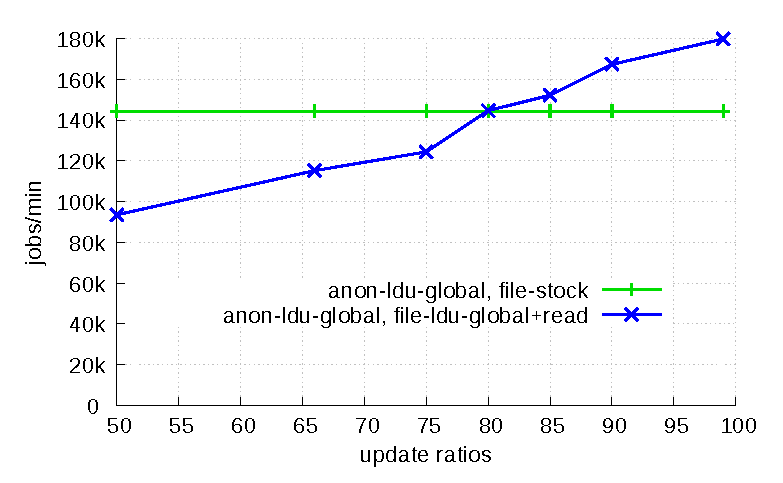
\includegraphics[height=2.5in]{graph/ratio_exim.eps}
        \caption{AIM7 - 120core}
  \end{center}
    \end{subfigure}%
    \caption{Performance depending on update ratios and scalability.}
    \label{fig:UpdateRate_exim}
\end{figure*}

\begin{figure*}[t!]
    \centering
    \begin{subfigure}[b]{1\textwidth}
        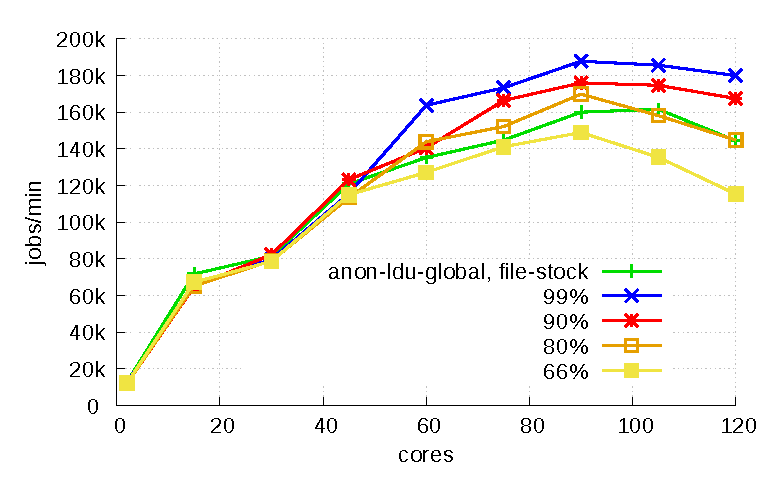
\includegraphics[height=2.5in]{graph/ratio_exim_core.eps}
        \caption{AIM7 - scalability}
    \end{subfigure}%
    \caption{Performance depending on update ratios and scalability.}
    \label{fig:UpdateRate_exim_2}
\end{figure*}

\begin{figure*}[t!]
    \centering
    \begin{subfigure}[b]{1\textwidth}
  \begin{center}
        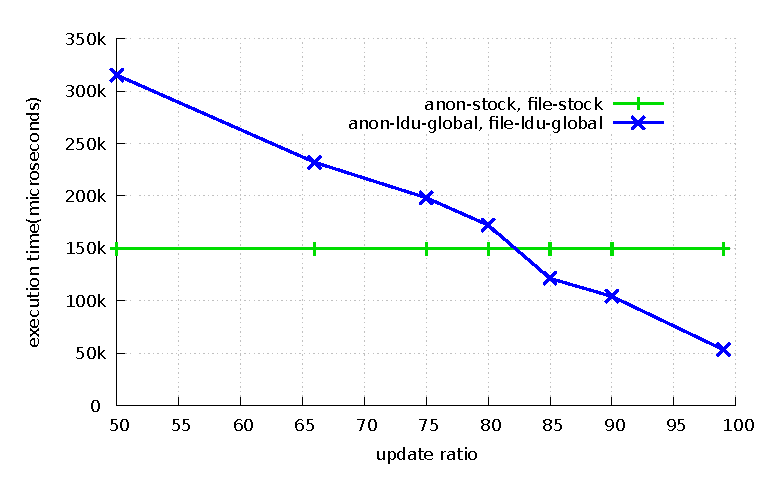
\includegraphics[height=2.5in]{graph/ratio_lmbench.eps}
        \caption{AIM7 - 120core}
  \end{center}
    \end{subfigure}%
    \caption{Performance depending on update ratios and scalability.}
    \label{fig:UpdateRate_lmbench}
\end{figure*}

\begin{figure*}[t!]
    \centering
    \begin{subfigure}[b]{1\textwidth}
        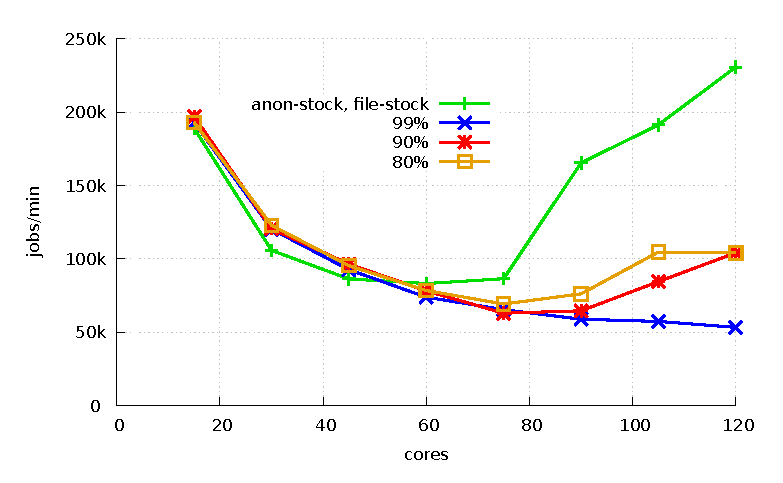
\includegraphics[height=2.5in]{graph/ratio_lmbench_core.eps}
        \caption{AIM7 - scalability}
    \end{subfigure}%
    \caption{Performance depending on update ratios and scalability.}
    \label{fig:UpdateRate_lmbench_2}
\end{figure*}


\subsection{Lmbench}
%$$$$$$$$$$$$$$$$$$$$$$$$$$$$$$$$$$$$$$$$$$$$$$$$$$$$$$$$$$$$$$$$$$$$$$$$$$$$$$$$
%Paragraph 1: %워크로드에 대한 설명
%$$$$$$$$$$$$$$$$$$$$$$$$$$$$$$$$$$$$$$$$$$$$$$$$$$$$$$$$$$$$$$$$$$$$$$$$$$$$$$$$
The Lmbench has various micro benchmarks including process management workloads.
We used the process management workload in the Lmbench.
This workload is used to measure the basic process primitives such as creating a
new process, running a program, and context switching.
We configured process create workload to enable the parallelism option(the
value was 1000).

%$$$$$$$$$$$$$$$$$$$$$$$$$$$$$$$$$$$$$$$$$$$$$$$$$$$$$$$$$$$$$$$$$$$$$$$$$$$$$$$$
%Paragraph 2: 실험 결과에 대한 설명
%$$$$$$$$$$$$$$$$$$$$$$$$$$$$$$$$$$$$$$$$$$$$$$$$$$$$$$$$$$$$$$$$$$$$$$$$$$$$$$$$
The results for the Lmbench are shown in Figure~\ref{fig:MicroBench}, 
and the results show the execution times.
Up to 45 core, the stock Linux scales linearly and then the execution time goes
up to grow.
The per-core version of the \LDU outperforms the stock Linux by 2.7x and the Harris by
1.1x at 120 core.
While the stock Linux has 69\% idle time, other methods have approximately 35\%
idle time since the stock Linux waits to acquire two rmap
semaphores(\code{anon\_vma->rwsem}, \code{mapping->i\_mmap\_rwsem})(see
figure~\ref{fig:utilization_lmbench}).
Indeed, our main motivation in the \LDU is to improve the performance and scalability on
the many-core systems, so we did not consider a low cores performance(under 30 cores).
However, up to 30 core, our \LDU is similar to the stock Linux performance, but
the Harris has low performance up to 60 core.

\subsection{Updates ratio}

%$$$$$$$$$$$$$$$$$$$$$$$$$$$$$$$$$$$$$$$$$$$$$$$$$$$$$$$$$$$$$$$$$$$$$$$$$$$$$$$$
%Paragraph 2:  실험을 수행한 이유
%$$$$$$$$$$$$$$$$$$$$$$$$$$$$$$$$$$$$$$$$$$$$$$$$$$$$$$$$$$$$$$$$$$$$$$$$$$$$$$$$
One question that could be raised regarding the proposed
\LDU scheme would be how the performance scalability is affected
by the frequency of read operations since the proposed technique
has only focused on update-heavy data structures with very low
read ratios.
Even read operations could be slower since read operation should
perform code{synchronize} function to apply logs.

To understand the effect of read operations, we performed another experiment with intentionally adding the read operations in proportion to update operations.
The anonymous rmap used the global queue version of the \LDU, and then we sequentially increased read (\code{lock},
\code{synchronize}) ratios regarding the file rmap.
The upper graphs of figure \ref{fig:UpdateRate_aim7} 
,\ref{fig:UpdateRate_aim7_2} ,  \ref{fig:UpdateRate_exim}, 
\ref{fig:UpdateRate_exim_2},  \ref{fig:UpdateRate_lmbench} and
\ref{fig:UpdateRate_lmbench_2} shows the performance on 120 core depending on
its update ratios, and the lower graphs represent the scalability.

%$$$$$$$$$$$$$$$$$$$$$$$$$$$$$$$$$$$$$$$$$$$$$$$$$$$$$$$$$$$$$$$$$$$$$$$$$$$$$$$$
%Paragraph 2: 실험 결과에 대한 설명
%$$$$$$$$$$$$$$$$$$$$$$$$$$$$$$$$$$$$$$$$$$$$$$$$$$$$$$$$$$$$$$$$$$$$$$$$$$$$$$$$
Since the AIM7 has less fork-intensive workload than other ones, the
read operations are invoked relatively infrequently.
As a result, although the data structure uses 75\% update rates(3 update, 1 read), 
the \LDU version of Linux has outstanding performance than stock Linux.
The scalability of AIM7 shows that the \LDU has substantially high scalability at the
the 90\% and the 99\% update rates as well as the 80\% update rates. 

%$$$$$$$$$$$$$$$$$$$$$$$$$$$$$$$$$$$$$$$$$$$$$$$$$$$$$$$$$$$$$$$$$$$$$$$$$$$$$$$$
%Paragraph 2: 실험 결과에 대한 설명
%$$$$$$$$$$$$$$$$$$$$$$$$$$$$$$$$$$$$$$$$$$$$$$$$$$$$$$$$$$$$$$$$$$$$$$$$$$$$$$$$
The Exim and the Lmbench show the extremely high fork-intensive workload.
As a result, the stock Linux outperforms the \LDU by approximately
80\%, but the \LDU outperforms the stock kernel after 85\%.
This explains the \LDU has outstanding performance even when the read operations 
frequently occur.
